% main.tex -- arXiv preprint (quant-ph). Compile: tectonic main.tex  (or pdflatex + bibtex + 2x pdflatex).
%
% Sources: REPORT.md, CERTIFICATES.md, code in pauli-emergence/ and
% depolarizing-threshold/ of the public repository. Every number below is taken from those files or from the logs in
% pauli-emergence/runs/ (checked 2026-10-12); derived constants were recomputed.
%
% Search for "PENDING" for statements whose final numbers may still change.
\documentclass[aps,pra,reprint,superscriptaddress,nofootinbib,longbibliography,floatfix]{revtex4-2}

\usepackage{amsmath,amssymb,amsthm}
\usepackage{graphicx}
\usepackage{xcolor}
\usepackage{tikz}
\usepackage[colorlinks=true,linkcolor=blue!60!black,citecolor=blue!60!black,urlcolor=blue!60!black]{hyperref}

\newtheorem{proposition}{Proposition}
\newtheorem{lemma}{Lemma}
\newtheorem{theorem}{Theorem}
\newtheorem{corollary}{Corollary}
\theoremstyle{remark}
\newtheorem{remark}{Remark}

\newcommand{\ket}[1]{\lvert #1\rangle}
\newcommand{\bra}[1]{\langle #1\rvert}
\newcommand{\Tr}{\operatorname{Tr}}
\newcommand{\diag}{\operatorname{diag}}
\newcommand{\id}{\mathrm{id}}
\newcommand{\one}{\openone}
\newcommand{\Ic}{I_c}
\newcommand{\lperp}{\lambda_\perp}
\newcommand{\lpar}{\lambda_\parallel}
\newcommand{\Sym}{\mathrm{Sym}}
\newcommand{\Nsig}{\mathcal{N}_\sigma}
\newcommand{\Amp}{\mathcal{A}}
\newcommand{\Loss}{\mathcal{L}}

\begin{document}

\title{Emergent Gaussian channels for Pauli noise: certified quantum-capacity thresholds and
positive capacity of the additive Gaussian noise channel beyond $1/\sqrt{e}$}

\author{Jimmy Kelvyn Estevam Carvalho}
\affiliation{RCO Tecnologia Ltda.}

\date{Draft of October 12, 2026}

\begin{abstract}
A qubit Pauli channel acting on permutation-symmetric states of $M$ qubits with a bounded number of
excitations around a pole of the Bloch sphere behaves, for large $M$, like a single-mode bosonic
Gaussian channel; Ahmed \textit{et al.}\ identified this emergent channel for the depolarizing
channel. We give its form for an arbitrary Pauli channel with Bloch factors
$(\lambda_a,\lambda_b,\lambda_c)$ and pole along $c$: $X=\diag(\lambda_a,\lambda_b)/\sqrt{\lambda_c}$ and
$Y=\diag(1-\lambda_a^2,1-\lambda_b^2)/(2\lambda_c)$. Its complete positivity is equivalent to the
nonnegativity of the Gram determinant $1-\lambda_a^2-\lambda_b^2-\lambda_c^2+2\lambda_a\lambda_b\lambda_c$.
For the independent $X$--$Z$ (BB84) channel the emergent channel is the additive Gaussian noise (AGN)
channel; for the 2-Pauli channel it is a quantum-limited amplifier after pure loss. The emergent
channel is antidegradable if and only if $\lperp\le 1/\sqrt2$, the shrinking factor of optimal
phase-covariant cloning, which caps what this route can certify. Using an exact band-decomposed
evolution in the Dicke basis and two interval-arithmetic certifiers, we certify positive coherent
information of explicit $M$-qubit states at $q=0.126$ for BB84 ($M=240$) and $p=0.1255$ for the
2-Pauli channel ($M=240$), above the previously reported $0.118371$ and $0.118067$, and at total error
$0.1977936$ for the depolarizing channel ($M=240$). In the Gaussian limit we certify the emergent
depolarizing channel at total error $0.1997875$; with the convergence theorem of Ahmed \textit{et al.}\
this is, to our knowledge, the largest depolarizing threshold bound whose final sign is certified (the
larger $0.2029161$ rests on a floating-point value $\Ic\approx10^{-12}$).
Transferring the BB84 code to the Gaussian limit, we certify
positive coherent information for the AGN channel at noise variance $\sigma^2=6579/16000$
($\sigma\approx0.6412$), hence positive quantum capacity for all $\sigma^2\le0.4111875$, beyond
$\sigma^2=1/e$ where the Gaussian-input coherent information vanishes; this refutes the 2001
speculation that the Gaussian-input coherent information is the capacity of this channel. For the thermal attenuator we certify $Q>0$ well inside the open window at every temperature tried
(e.g.\ $\eta\ge0.78$ with one thermal photon, below the recently certified $0.7841$).
All results are computer-assisted; human verification is pending.
\end{abstract}

\maketitle

% =====================================================================================================
\section{Introduction}
\label{sec:intro}

The quantum capacity of a channel $\mathcal N$ is its regularized coherent
information~\cite{lloyd1997capacity,devetak2005private},
\begin{equation}
  Q(\mathcal N)=\lim_{n\to\infty}\frac1n\max_\rho \Ic(\rho,\mathcal N^{\otimes n}),
  \label{eq:Q}
\end{equation}
with $\Ic(\rho,\mathcal N)=S(B)-S(RB)$,
where $S(B)=S(\mathcal N(\rho))$, $S(RB)=S((\id_R\otimes\mathcal N)(\psi_\rho))$ and $\psi_\rho$ purifies
$\rho$. Any explicit input $\rho$ on $M$ channel uses with $\Ic(\rho,\mathcal N^{\otimes M})>0$
certifies $Q(\mathcal N)\ge \Ic/M>0$. For a one-parameter noise family $\mathcal N_p$ we write
$p_{\mathrm{th}}=\sup\{p:Q(\mathcal N_p)>0\}$. Because the maximal coherent information can be
strictly superadditive~\cite{divincenzo1998verynoisy}, $p_{\mathrm{th}}$ can lie above the hashing
point~\cite{bennett1996mixed}, where the single-letter coherent information of the maximally mixed
input vanishes; the improvements come from degenerate
codes~\cite{divincenzo1998verynoisy,smith2007degenerate,fern2008lower,bausch2021pauli}.

We consider qubit Pauli channels
$\mathcal N(\rho)=p_I\rho+p_XX\rho X+p_YY\rho Y+p_ZZ\rho Z$ and three standard families:
the depolarizing channel $(p_I,p_X,p_Y,p_Z)=(1-3p,p,p,p)$, whose total error is $3p$; the
independent $X$--$Z$ channel, also called the BB84 channel, $((1-q)^2,q(1-q),q^2,q(1-q))$; and the
2-Pauli channel $(1-2p,p,0,p)$. Their hashing points are $3p=0.189290$, $q=0.110028$ and $p=0.113546$.

\paragraph*{State of the art.}
Bhalerao and Leditzky~\cite{bhalerao2025permutation} introduced representation-theoretic methods for
permutation-invariant codes. Agarwal \textit{et al.}~\cite{agarwal2026symmetry} extended them to rank-two
states on the full symmetric subspace and reported $q=0.118371$ (BB84) and $p=0.118067$ (2-Pauli) at
input length $n=30$, and $p=0.064657$ per Pauli for the depolarizing channel at $n=45$.
Krohn-Grimberghe~\cite{krohn2026certified} gave exact-arithmetic, independently machine-checkable
positivity proofs for the depolarizing channel, at $p=16239/250000$ per Pauli ($3p=0.194868$, $n=45$), and noted
that the final sign evaluation of earlier reported thresholds was done in floating point. Ahmed
\textit{et al.}~\cite{ahmed2026choir} showed that the depolarizing channel, acting on symmetric states
with a bounded number of excitations, converges to a bosonic thermal attenuator; optimizing residue
(cat-like) codes for that Gaussian channel and using a convergence theorem (their Theorem~6), they
obtained $p_{\mathrm{th}}\gtrsim 0.2029161$ in total error (transmissivity $\eta=0.7294452$), valid for
sufficiently large $M$, with a reported Gaussian-channel coherent information
$\Ic\approx10^{-12}$ at that point. Table~\ref{tab:overview} summarizes.

\paragraph*{The additive Gaussian noise channel.}
The AGN channel $\Nsig$ (also called the Gaussian random displacement or classical-noise channel)
displaces both quadratures by independent Gaussian noise of variance $\sigma^2$, in units where the
vacuum variance is $1/2$. Its quantum capacity is unknown. Thermal (Gaussian) inputs give
$Q(\Nsig)\ge\max\{0,\log_2[1/(e\sigma^2)]\}$~\cite{holevo2001evaluating}, a rate that
Gottesman--Kitaev--Preskill (GKP) lattice codes can match~\cite{harrington2001achievable}; the channel
is antidegradable, hence $Q=0$, for
$\sigma^2\ge1/2$~\cite{caruso2006degradability,lami2019extendibility}. Lin and
Noh~\cite{lin2025gkp} decoded multi-mode GKP codes with exact or approximate maximum-likelihood
decoders: the $d=39$ surface-square code keeps a nonzero rate up to $\sigma=0.598$, the threshold of
the surface-square family is close to $1/\sqrt e\simeq0.6065$, and they discuss the prospect of a nonzero rate in the window
$1/\sqrt e\le\sigma<1/\sqrt2$, where no positive lower bound was known. Zhang, Wu and Guo~\cite{zhang2023xzzx}
reported a code-capacity threshold $\sigma\approx0.67$ for rectangular GKP codes concatenated with the
XZZX surface code, from simulations with minimum-weight matching up to distance~9; Lin and Noh found
that the crossing points drift downward with the distance and concluded that this does not establish a
threshold above $1/\sqrt e$~\cite{lin2025gkp}. Such simulations are not proofs. Harrington and
Preskill, observing that GKP rates match the Gaussian-input coherent information, wrote that ``it is
tempting to speculate that this optimal one-shot coherent information actually is the quantum capacity
of the channel''~\cite{harrington2001achievable}. The closest related work is
by Mele \textit{et al.}~\cite{mele2026thermal}, who prove that non-Gaussian inputs beat the
Holevo--Werner thermal-state bound for the thermal attenuator.

\begin{table}[t]
\caption{Lower bounds on $p_{\mathrm{th}}$. ``This work'' entries are certified for an explicit state
(Sec.~\ref{sec:results}); the last column is the ceiling of the Gaussian-limit route
(Sec.~\ref{sec:ceiling}). For the AGN channel the parameter is $\sigma^2$ and ``hashing'' is the
Gaussian-input value.}
\label{tab:overview}
\begin{ruledtabular}
\begin{tabular}{lllll}
channel & hashing & previous best & this work & ceiling\\
\hline
BB84 ($q$) & 0.110028 & 0.118371~\cite{agarwal2026symmetry} & 0.126 & 0.146447\\
2-Pauli ($p$) & 0.113546 & 0.118067~\cite{agarwal2026symmetry} & 0.1255 & 0.146447\\
depol.\ ($3p$) & 0.189290 & 0.2029161$^{a}$~\cite{ahmed2026choir} & 0.1997875$^{b}$ & 0.219670\\
AGN ($\sigma^2$) & $1/e$ & $1/e$~\cite{holevo2001evaluating} & $0.4111875$ & $1/2$\\
\end{tabular}
\end{ruledtabular}
\raggedright\footnotesize
$^{a}$Gaussian limit with a convergence theorem, $M$ sufficiently large; the best previous certified
value for an explicit size is $0.194868$ ($n=45$)~\cite{krohn2026certified}.\\
$^{b}$Gaussian limit with $\Ic$ certified (Sec.~\ref{sec:depgauss}) and the convergence theorem of
Ref.~\cite{ahmed2026choir}, $M$ sufficiently large; the best explicit-size certificate is $0.1977936$
($M=240$).
\end{table}

\paragraph*{Contributions.}
(i) We give the emergent Gaussian channel of an arbitrary Pauli channel (Sec.~\ref{sec:emergent}), show
that its complete positivity is the nonnegativity of a Gram determinant, and identify the BB84 and
2-Pauli cases. (ii) We show that the emergent channel is antidegradable exactly when
$\lperp\le1/\sqrt2$ (Sec.~\ref{sec:ceiling}). (iii) We describe an exact finite-$M$ method
(Sec.~\ref{sec:finite}) and two rigorous certifiers based on ball arithmetic (Sec.~\ref{sec:certify}).
(iv) We certify thresholds for the BB84, 2-Pauli and depolarizing channels and for a family between the
last two (Sec.~\ref{sec:results}). (v) We certify $Q(\Nsig)>0$ for $\sigma^2\le0.4111875$
(Sec.~\ref{sec:agn}). Section~\ref{sec:failures} lists what did not work, Sec.~\ref{sec:open} open
problems and Sec.~\ref{sec:repro} how to reproduce every certificate.

\paragraph*{Status.}
The emergent-channel formula is derived from first and second moments; its Gaussianity is proven only
for the depolarizing channel~\cite{ahmed2026choir} and is supported here numerically. The thresholds
of Sec.~\ref{sec:results} and the AGN result use no limit theorem: each is a finite computation with
rigorous error control. They were checked by two independent code reviews and, for the AGN result, by
an independent re-implementation, all carried out by separate instances of an AI system
(see Acknowledgments). Independent human verification is pending.

% =====================================================================================================
\section{Emergent Gaussian channel of a Pauli channel}
\label{sec:emergent}

\subsection{Setting}
A Pauli channel shrinks the Bloch vector along the coordinate axes by the factors
\begin{equation}
  \lambda_x=1-2(p_Y+p_Z)\quad\text{and cyclic permutations.}
\end{equation}
Let $(a,b,c)$ be a permutation of $(x,y,z)$ with $\lambda_c>0$; the axis $c$ will be the pole. Let
$J_a=\tfrac12\sum_i\sigma_a^{(i)}$ be the collective spin of $M$ qubits and $\ket{J,m}$ the Dicke states
with $m$ measured along $c$. Symmetric inputs live in the $J=M/2$ block, and
$\ket{M/2,M/2-k}$ has $k$ excitations below the pole. For $k\ll M$ the Holstein--Primakoff
map~\cite{holstein1940} $J_-\simeq\sqrt{2J}\,b$ identifies $\ket{M/2,M/2-k}$ with the Fock state
$\ket k$ of a mode $b$, with quadratures $x=(b+b^\dagger)/\sqrt2$, $p=i(b^\dagger-b)/\sqrt2$ and vacuum
variance $1/2$.

The output $\mathcal N^{\otimes M}(\rho)$ of a symmetric input is permutation invariant, so by
Schur--Weyl duality
\begin{equation}
\begin{split}
  \mathcal N^{\otimes M}(\rho)&=\bigoplus_J B_J\otimes\frac{\one_{d_J}}{d_J},\\
  (\id_R\otimes\mathcal N^{\otimes M})(\psi_\rho)&=\bigoplus_J (RB)_J\otimes\frac{\one_{d_J}}{d_J},
\end{split}
  \label{eq:schurweyl}
\end{equation}
where $d_J$ is the multiplicity of spin $J$ and $B_J$ carries the full weight of sector $J$. The
multiplicity terms $\Tr(B_J)\log d_J$ appear identically in $S(B)$ and $S(RB)$, so
\begin{equation}
  \Ic(\rho,\mathcal N^{\otimes M})=\sum_J\bigl[S(B_J)-S((RB)_J)\bigr].
  \label{eq:blockIc}
\end{equation}
For inputs with few excitations the output weight concentrates at $J\simeq\lambda_cM/2$. In each sector
we use the Holstein--Primakoff mode around the same pole.

\subsection{Moment formula}
We use the conventions of Ref.~\cite{holevo2007onemode}: a single-mode Gaussian channel acts on the
mean vector $d$ and covariance matrix $V$ as $d\mapsto Xd$, $V\mapsto XVX^{\mathsf T}+Y$, and it is
completely positive if and only if
\begin{equation}
  Y+\tfrac i2\,(\Omega-X\Omega X^{\mathsf T})\succeq0,\qquad \Omega=\begin{pmatrix}0&1\\-1&0\end{pmatrix}.
  \label{eq:cp}
\end{equation}
Pure loss $\Loss_T$ has $X=\sqrt T\one$, $Y=\frac{1-T}2\one$; the quantum-limited amplifier $\Amp_G$ has
$X=\sqrt G\one$, $Y=\frac{G-1}2\one$; the AGN channel $\Nsig$ has $X=\one$, $Y=\sigma^2\one$.

\begin{proposition}[Emergent channel; moment formula]
\label{prop:emergent}
For inputs supported on a fixed number of excitations around the pole $c$, the first and second moments
of the renormalized output mode, sector by sector, converge as $M\to\infty$ to those of the Gaussian
channel
\begin{equation}
  X=\frac{1}{\sqrt{\lambda_c}}\diag(\lambda_a,\lambda_b),\qquad
  Y=\frac{1}{2\lambda_c}\diag(1-\lambda_a^2,\,1-\lambda_b^2).
  \label{eq:XY}
\end{equation}
\end{proposition}

\textit{Derivation.} (i) First moments. In the Heisenberg picture $\mathcal N^\dagger(\sigma_a)=\lambda_a\sigma_a$,
so $\langle J_a\rangle\mapsto\lambda_a\langle J_a\rangle$. With $J_a\simeq\sqrt{J}\,x$ in a sector of
spin $J$, $J_{\mathrm{in}}=M/2$ and $J_{\mathrm{out}}\simeq\lambda_cM/2$, this gives
$x\mapsto(\lambda_a/\sqrt{\lambda_c})\,x$ and likewise $p\mapsto(\lambda_b/\sqrt{\lambda_c})\,p$.
(ii) Second moments. The vacuum (all spins at the pole) is mapped to the product state
$\bigl[\tfrac12(\one+\lambda_c\sigma_c)\bigr]^{\otimes M}$. Inside each spin-$J$ sector this state is
proportional to $r^{k}$, with $k=J-m$ and $r=(1-\lambda_c)/(1+\lambda_c)$. This is a truncated geometric
distribution with mean $r/(1-r)=(1-\lambda_c)/(2\lambda_c)$, that is, a thermal state with isotropic
quadrature variance $1/(2\lambda_c)$. Then $Y=V_{\mathrm{out}}(\text{vac})-\tfrac12XX^{\mathsf T}$ gives
Eq.~\eqref{eq:XY}. \qed

The formula fixes the channel once the limit is known to be Gaussian. Ahmed
\textit{et al.}\ proved this for the depolarizing channel~\cite{ahmed2026choir}. For other Pauli
channels we have no proof; the exact computations of Table~\ref{tab:validation} support it
(Sec.~\ref{sec:validation}).

\begin{lemma}[Complete positivity]
\label{lem:gram}
For the pair~\eqref{eq:XY}, condition~\eqref{eq:cp} is equivalent to
\begin{equation}
  \Delta:=1-\lambda_a^2-\lambda_b^2-\lambda_c^2+2\lambda_a\lambda_b\lambda_c\ \ge 0,
  \label{eq:gram}
\end{equation}
which holds for every Pauli channel.
\end{lemma}
\begin{proof}
For $2\times2$ matrices $\Omega-X\Omega X^{\mathsf T}=(1-\det X)\Omega$, so Eq.~\eqref{eq:cp} reads
$Y\succeq0$ and $\det Y\ge\frac14(1-\det X)^2$. With Eq.~\eqref{eq:XY} the latter is
$(1-\lambda_a^2)(1-\lambda_b^2)\ge(\lambda_c-\lambda_a\lambda_b)^2$, which is $\Delta\ge0$; $Y\succeq0$
holds since $|\lambda_a|,|\lambda_b|\le1$. $\Delta$ is the determinant of the correlation (Gram) matrix
$C=\bigl(\begin{smallmatrix}1&\lambda_c&\lambda_b\\ \lambda_c&1&\lambda_a\\ \lambda_b&\lambda_a&1\end{smallmatrix}\bigr)$.
$C$ is affine in the Pauli probabilities, and at the four Pauli channels
$\rho\mapsto P\rho P$ it equals $vv^{\mathsf T}$ with $v\in\{\pm1\}^3$. For example, $P=X$ gives
$(\lambda_x,\lambda_y,\lambda_z)=(1,-1,-1)$ and $v=(1,-1,-1)$. Hence
$C=\sum_Pp_Pv_Pv_P^{\mathsf T}\succeq0$ and $\Delta=\det C\ge0$.
\end{proof}

\subsection{Special cases}
\label{sec:special}
\paragraph*{Depolarizing.} $\lambda_a=\lambda_b=\lambda_c=\eta=1-4p$ gives $X=\sqrt\eta\one$ and
$Y=(1-\eta^2)/(2\eta)\one=(1-\eta)(N_E+\frac12)\one$ with $N_E=1/(2\eta)$. This is the thermal attenuator
of Ahmed \textit{et al.}, which they write as $\Amp_G\circ\Loss_T$ with $T=2\eta^2/(1+\eta)$ and
$G=(1+\eta)/(2\eta)$~\cite{ahmed2026choir}.

\paragraph*{Phase-covariant channels.} If $\lambda_a=\lambda_b=\lperp$ and $\lambda_c=\lpar$ (pole on the
axis of phase covariance), the emergent channel is phase insensitive, with
\begin{equation}
  \tau=\frac{\lperp^2}{\lpar},\qquad Y=\frac{1-\lperp^2}{2\lpar}.
  \label{eq:tauY}
\end{equation}
Every such channel equals $\Amp_G\circ\Loss_T$ with $G=Y+(1+\tau)/2$ and $T=\tau/G$.

\paragraph*{BB84.} With the pole on $y$: $\lambda_x=\lambda_z=s:=1-2q$ and $\lambda_y=s^2$. Then
$\tau=1$, and the emergent channel is the AGN channel with
\begin{equation}
  \sigma^2=Y=\frac{1-s^2}{2s^2}=\frac{1-(1-2q)^2}{2(1-2q)^2}.
  \label{eq:sigmaq}
\end{equation}
The map $q\mapsto\sigma^2$ is increasing. Gaussian inputs stop at $\sigma^2=1/e$, i.e.\ $q=0.120488$;
antidegradability starts at $\sigma^2=1/2$, i.e.\ $q=0.146447$; and $\sigma^2=2/5$ corresponds to
$q=0.127322$.

\paragraph*{2-Pauli.} With the pole on $y$: $\lambda_x=\lambda_z=1-2p$ and $\lambda_y=1-4p$, so
$\tau=(1-2p)^2/(1-4p)>1$ and $Y=2p(1-p)/(1-4p)$. This is $\Amp_G\circ\Loss_T$ with $T=1-2p$ and
$G=(1-2p)/(1-4p)$, a quantum-limited amplifier after pure loss.

\begin{remark}[A heuristic mechanism]
\label{rem:mechanism}
With the pole on the phase-covariance axis, a unital phase-covariant Pauli channel is the mixture
\begin{equation}
  \mathcal N=\lperp\,\id+(\lperp-\lpar)\,F+(1-2\lperp+\lpar)\,R
\end{equation}
whenever the coefficients are nonnegative. Here $R(\rho)=\Tr\rho\,\one/2$ and
$F(\rho)=\frac12(\sigma_a\rho\sigma_a+\sigma_b\rho\sigma_b)$ (``measure $\sigma_c$, then flip''). BB84
has coefficients $(s,\,s(1-s),\,(1-s)^2)$ and 2-Pauli has $(1-2p,\,2p,\,0)$. Apply $F$ to a random
fraction $f$ of the qubits of a symmetric state with few excitations. It removes the excitations it
finds, which acts as pure loss with $T=1-f$, and it appends a block polarized toward the opposite pole.
After recoupling to the total spin, the Holstein--Primakoff mode of that block enters phase-conjugated,
which acts as a quantum-limited amplifier with $G=(1-f)/(1-2f)$. For $f=2p$ this gives the 2-Pauli
emergent channel above. It is the analogue of the ``loss plus universal cloning'' decomposition on which
the depolarizing proof of Ref.~\cite{ahmed2026choir} rests (their Theorem~2), with the cloner replaced by
coupling to a flipped block. We do not turn this into a proof here.
\end{remark}

\subsection{Numerical validation}
\label{sec:validation}
Table~\ref{tab:validation} compares the exact $M$-qubit coherent information (Sec.~\ref{sec:finite},
double precision) for thermal (geometric) weights on the Dicke ladder of the BB84 channel with the
prediction of the emergent channel. The gap decays as $c/M$ with $c\approx1.25\,\bar n$, and Richardson
extrapolation of the $q=0.1184$ column gives $+0.0080$, against the predicted $+0.0077$. These numbers are
floating-point evidence for Proposition~\ref{prop:emergent}, not certificates.

\begin{table}[t]
\caption{BB84 channel, thermal input with mean excitation $\bar n$ on the Dicke ladder (truncated):
exact $\Ic$ (bits) of the $M$-qubit state versus the emergent-channel prediction (double precision;
not certified).}
\label{tab:validation}
\begin{ruledtabular}
\begin{tabular}{lll}
$M$ & $q=0.10$, $\bar n=1$ & $q=0.1184$, $\bar n=4$\\
\hline
8 & 0.0922 & \\
16 & 0.1203 & \\
32 & 0.1427 & \\
64 & 0.1546 & $-0.0711$\\
128 & & $-0.0314$\\
256 & & $-0.0117$\\
Richardson ($M\to\infty$) & & $+0.0080$\\
emergent channel & 0.1668 & $+0.0077$\\
\end{tabular}
\end{ruledtabular}
\end{table}

% =====================================================================================================
\section{Ceiling of the Gaussian route}
\label{sec:ceiling}

\begin{lemma}
\label{lem:antideg}
A phase-insensitive single-mode Gaussian channel with transmissivity or gain $\tau>0$ and added noise
$Y$ (vacuum variance $1/2$) is antidegradable if and only if $Y\ge\tau/2$.
\end{lemma}
\begin{proof}
Lami \textit{et al.}~\cite{lami2019extendibility} give necessary and sufficient conditions for
two-extendibility, i.e.\ antidegradability, of the three classes, recovering
Ref.~\cite{caruso2006degradability}. In our units: thermal attenuator, $Y=(1-\tau)(N+\frac12)$, iff
$\tau\le(N+\frac12)/(N+1)$; amplifier, $Y=(\tau-1)(N+\frac12)$, iff $\tau\ge(N+\frac12)/N$; additive noise
($\tau=1$) iff $Y\ge\frac12$. Substituting $N$, each condition is $Y\ge\tau/2$.
\end{proof}

\begin{corollary}
\label{cor:ceiling}
The emergent channel~\eqref{eq:tauY} of a phase-covariant Pauli channel is antidegradable if and only if
$\lperp\le1/\sqrt2$, independently of $\lpar$.
\end{corollary}
\begin{proof}
$(1-\lperp^2)/(2\lpar)\ge\lperp^2/(2\lpar)\iff\lperp^2\le\frac12$.
\end{proof}

The value $1/\sqrt2$ is the shrinking factor of the optimal phase-covariant $1\to2$ qubit cloner
(fidelity $\frac12+\sqrt{1/8}$)~\cite{bruss2000phasecovariant}. Codes analysed through the emergent
channel, i.e.\ with a bounded number of excitations near one pole as $M\to\infty$, therefore cannot
certify $Q>0$ beyond the phase-covariant cloning point. For BB84 and 2-Pauli this point is
$q,p=(1-1/\sqrt2)/2=0.146447$, the familiar 14.6\% error rate of the phase-covariant cloning attack on
BB84~\cite{bruss2000phasecovariant}. For the depolarizing channel it is
$3p=\frac34(1-1/\sqrt2)=0.219670$, below the true antidegradability point $3p=1/4$ set by universal
cloning. For the AGN channel it is $\sigma^2=1/2$. Explicit finite-$M$ states are not bound by this
ceiling.

For phase-covariant noise with the pole on the third axis, the ceiling exceeds the hashing point only
when the noise along the pole is not too large. Table~\ref{tab:bias} shows this for $Z$-biased noise
$(p_X,p_Y,p_Z)=p\,(\frac1{2(b+1)},\frac1{2(b+1)},\frac{b}{b+1})$ with the pole on $z$: the route is
useless for $b\gtrsim1$ and useful between the 2-Pauli ($b=0$) and depolarizing ($b=\frac12$) channels.

\begin{table}[t]
\caption{$Z$-biased Pauli noise with total error $p$ and pole on $z$: hashing point, the Gaussian-route
threshold with thermal inputs at infinite energy (closed form, Holevo--Werner
type~\cite{holevo2001evaluating}), and the ceiling of Corollary~\ref{cor:ceiling}.}
\label{tab:bias}
\begin{ruledtabular}
\begin{tabular}{llll}
bias $b$ & hashing & Gaussian inputs & ceiling\\
\hline
0 (2-Pauli type) & 0.22709 & 0.24149 & 0.29289\\
0.25 & 0.19260 & 0.20214 & 0.24408\\
0.5 (depolarizing) & 0.18929 & 0.18470 & 0.21967\\
1 & 0.19378 & 0.16856 & 0.19526\\
3 & 0.22221 & 0.15234 & 0.16737\\
10 & 0.27791 & 0.14643 & 0.15342\\
\end{tabular}
\end{ruledtabular}
\end{table}

% =====================================================================================================
\section{Exact finite-$M$ computation}
\label{sec:finite}

\paragraph*{Generator.} With the pole on the phase-covariance axis $c$ (the $y$ axis for BB84 and
2-Pauli, the $z$ axis for the depolarizing channel and the family of Sec.~\ref{sec:family}), the channel
is unital and phase covariant, and
\begin{equation}
  \mathcal N=e^{\mathcal L},\quad
  \mathcal L=g\,\mathcal D[\sigma_-]+g\,\mathcal D[\sigma_+]+\tfrac{\gamma_D}{4}\,\mathcal D[\sigma_c],
  \label{eq:lindblad}
\end{equation}
with $g=-\tfrac12\ln\lpar$ and $\gamma_D=-2\ln\lperp+\ln\lpar$, where $\sigma_\pm$ raise and lower
along $c$. For 2-Pauli $\gamma_D<0$: $\mathcal L$ is then not a Lindbladian, but $e^{\mathcal L}$ is still
the CPTP map $\mathcal N$. On $M$ qubits $\mathcal N^{\otimes M}=\exp(\sum_i\mathcal L_i)$.

\paragraph*{Dicke basis and bands.} On permutation-invariant operators,
$\sum_i\mathcal L_i$ acts on the coefficients of $\ket{J,m}\bra{J,m'}$ through the closed-form
coefficients of the PIQS method~\cite{shammah2018piqs}. Each $J$ couples only to $J$ and $J\pm1$. In our
installation of \texttt{qutip.piqs}~\cite{johansson2013qutip} these coefficients came out with
single-precision accuracy (relative error $\sim10^{-8}$). We therefore reimplemented them in double
precision and, for the certificates, in ball arithmetic. Phase covariance conserves $\delta=m-m'$, so
each band $\delta$ is an invariant subspace of dimension $\sum_J(2J+1-\delta)\approx M^2/4$, instead of
the $\sim M^3/6$ of the full permutation-invariant operator space.

\paragraph*{Codes and coherent information.} The input is a rank-two state
$\rho=(\ket{\phi_0}\bra{\phi_0}+\ket{\phi_1}\bra{\phi_1})/Z$ in the $J=M/2$ block, with unnormalized
codewords $\phi_i=\sum_{k\le K}c_i(k)\ket{M/2,M/2-k}$. We use residue codes: $c_i(k)=0$ unless
$k\equiv a_i\pmod{\kappa}$, with $\kappa=2$ (parity) or $3$ and $(a_0,a_1)=(0,1)$. Because the channel
is linear, the outputs of all $\ket k\bra l$ with $k,l\le K$ are computed once, band by band, and every
input is evaluated by contraction. The phase covariance makes $B_J$ block diagonal in $x\bmod\kappa$
($x$ = excitations from the top of the spin-$J$ block) and $(RB)_J$ block diagonal in
$(x-a_i)\bmod\kappa$, and $\Ic$ follows from Eq.~\eqref{eq:blockIc}. Nothing is truncated: $\Sym^M$ and
all output sectors are finite dimensional.

\paragraph*{Optimization and validation.} Real amplitudes are optimized with L-BFGS using exact
gradients obtained from the adjoint map. Thresholds are located by continuation and bisection in $p$,
with warm starts and the criterion $\Ic>10^{-6}$ bits. The band evolution agrees with brute-force
$2^M$ simulation of random rank-two inputs for $M=3,\dots,6$ (BB84, depolarizing and 2-Pauli) to
$|\Delta\Ic|\le1.5\times10^{-15}$. From a parity-code start at $n=30$ the optimizer finds $\Ic>0$ at $q=0.1185$ (BB84) and $p=0.118$
(2-Pauli), consistent with Ref.~\cite{agarwal2026symmetry}. At the 2-Pauli and BB84 $M=60$ threshold
points, an independent evaluation with \texttt{qutip.piqs} gives $\Ic$ about $1\times10^{-7}$ below
ours, a difference explained by the single-precision coefficients.

% =====================================================================================================
\section{Rigorous certification}
\label{sec:certify}

Every certified point uses an exact rational noise parameter (e.g.\ $q=63/500$), hence rational Bloch
factors. The stored float64 amplitudes are read as exact dyadic rationals, so each certificate concerns
one exactly specified state. Certifier B rejects inputs with weight off the declared residues or with
$K>M$; for the inputs of certifiers F and L the exact-zero residue pattern was checked separately. Ball (midpoint--radius) arithmetic is provided by Arb~\cite{johansson2017arb} through
python-flint~0.9.0~\cite{pythonflint}.

\paragraph*{Entropy enclosure (both certifiers).} Let $A$ be a ball matrix that contains a density block
(of $B_J$ or $(RB)_J$, in one residue sector). Take a floating-point approximate eigenbasis $V$, read
exactly, and form $A'=V^{\mathsf T}AV=\diag(d)+E$ in ball arithmetic. Weyl's inequality gives
$|\lambda_i(A')-d_{(i)}|\le\|E\|_F$. Ostrowski's theorem~\cite{hornjohnson2012} gives
$\lambda_i(A')=\theta_i\lambda_i(A)$ with $|\theta_i-1|\le\delta$, where
$\delta\ge\|V^{\mathsf T}V-\one\|_F$ and $\delta<\frac12$ is checked. Since the true block is positive
semidefinite, every eigenvalue is enclosed in an interval in $[0,\infty)$, and
$h(t)=-t\ln t$, monotone on $[0,1/e]$ and on $[1/e,1]$, gives a rigorous interval for the entropy.

\paragraph*{Certifier F (\texttt{certify\_finite.py}).} All generator entries, including the rates
$-\frac12\ln\lambda$ and square roots, are Arb balls (160 bits). Each band is exponentiated with
\texttt{arb\_mat.exp}, which returns a rigorous enclosure. The blocks are assembled in ball arithmetic and
then enclosed as above. The cost is $\sim n^3$ per band of size $n$: $2.5\times10^3$\,s for BB84 at
$M=60$, practical up to $M\approx60$.

\paragraph*{Certifier B (\texttt{certify\_big.py}).} This certifier integrates the band ODE $v'=Lv$ in
floating point with a rigorous a~posteriori budget in the 1-norm. All bounds below are per column of the
propagated input operators.
\begin{enumerate}
\item \emph{Generator.} The entries of $L$ are Arb balls (128 bits), and the float matrix is
$L_f=\mathrm{fl}(\mathrm{mid}\,L)$, with $|L_f-L|\le\mathrm{rad}+u|L_f|$ entrywise. This yields rigorous
bounds on $\|L-L_f\|_1$, $\|L_f\|_1$ and the logarithmic norm
$\mu_1(L_f)=\max_c\bigl(L_{f,cc}+\sum_{r\ne c}|L_{f,rc}|\bigr)$~\cite{soderlind2006lognorm}, so that
$\|e^{tL_f}\|_1\le e^{t\max(\mu_1,0)}$.
\item \emph{Integration.} $e^{L_f}=(e^{hL_f})^s$ with $h=2^{-k}$ and $h\|L_f\|_1\le\frac14$
(cf.\ Ref.~\cite{almohy2011action}). Each step is a degree-16 Taylor sum. The budget bounds the
truncation (series tail, doubled), the rounding of every sparse product, $\gamma_q|L_f||t|$ with $q$ the
maximal number of nonzeros per row plus one~\cite{higham2002accuracy}, propagated through the remaining
Taylor recursion, and the rounding of the summation. Step errors are propagated to $t=1$ with
$e^{h\max(\mu_1,0)}$ per step.
\item \emph{Model error.} Duhamel's formula gives
$\|e^{L}-e^{L_f}\|_1\le e^{\max(\mu_1(L),\mu_1(L_f),0)}\|L-L_f\|_1$, with
$\mu_1(L)\le\mu_1(L_f)+\|L-L_f\|_1$.
\item \emph{Assembly and entropy.} The float blocks $\sigma$ are exact dyadic matrices. Their distance to
the true blocks is at most $\varepsilon$ in total absolute entry sum, hence in trace norm. Here
$\varepsilon$ is the sum of all terms above, weighted by $|c_a(k)c_b(l)|$, plus the assembly rounding,
divided by a lower bound on $Z$. The entropy of $\sigma$ is enclosed as above. With the negative
eigenvalues of $\sigma$ clipped, the true spectrum is within $\varepsilon'=\varepsilon+{}$(negative
mass) in $\ell_1$, and the continuity bound $|\sum h(\lambda_i)-\sum h(x_i)|\le\varepsilon'\ln(D/\varepsilon')$
for $\varepsilon'\le1/e$ (cf.\ Ref.~\cite{fannes1973continuity}) closes the interval, with $D$ the total
number of eigenvalues. A factor of 2 is applied to all budget totals.
\end{enumerate}
For BB84 and the depolarizing channel the band generators have $\mu_1\le0$, so the evolution contracts
in these coordinates. For 2-Pauli $\gamma_D<0$, and $\mu_1$ grows roughly linearly with $M$
($\approx3.2$, $6.8$, $10.6$, $14$ at $M=60,120,180,240$), so float64 rounding can be amplified by up
to $e^{\mu_1}$. Certifier~B was validated against certifier~F on the three $M=60$ states: the
intervals of~B contain those of~F. At $M=240$ it took $4.3\times10^3$\,s (depolarizing) and
$8.0\times10^3$\,s (BB84) of wall time on a 4-core x86-64 machine.

\paragraph*{Extended precision and a self-found bug.} With \texttt{CERT\_LD=1} the integration runs in
x87 extended precision ($u=2^{-64}$). The certifier refuses this mode unless
\texttt{numpy.longdouble} has a 64-bit mantissa. At $M=60$ this mode gives
$[4.4142155,4.4142560]\times10^{-6}$ for the 2-Pauli state, about $10^3$ times tighter than float64 and
containing the Arb-exponential interval. A self-audit found that the first version of this mode formed
the Taylor step scalar $h/n$ as a float64 quotient. That rounding, of relative size up to $2^{-53}$, was
not covered by the $2^{-64}$ budget. The scalar is now formed in extended precision, and the fix was made
before any extended-precision result entered the manifest. The $M=60$ cross-check was repeated after
the fix, with an interval containing the Arb-exponential one, and the two $M=180$ runs started with the
faulty version were discarded. Float64 mode was not affected, because its $4u$ term covers that
rounding.

\paragraph*{Certifier L (\texttt{certify\_limit.py}, bosonic).} For channels $\Amp_G\circ\Loss_T$ with
exact rational $T,G$, the Fock-basis band matrix elements
\begin{gather*}
  \Loss_T(\ket m\bra{m+d})=\textstyle\sum_k\ell_k\,\ket{m-k}\bra{m-k+d},\\
  \ell_k=\sqrt{\tbinom mk\tbinom{m+d}k}\,T^{m+\frac d2-k}(1-T)^k,\\
  \Amp_G(\ket j\bra{j+d})=\textstyle\sum_k a_k\,\ket{j+k}\bra{j+k+d},\\
  a_k=\sqrt{\tbinom{j+k}k\tbinom{j+d+k}k}\,(1-G^{-1})^k\,G^{-(j+\frac d2+1)},
\end{gather*}
are evaluated in Arb (192 bits) for inputs supported on $n\le N_{\mathrm{in}}$. Output levels above $D$
are collapsed into a flag state $\ket\perp$: $\mathcal T_D(\omega)=P\omega P+\Tr[(\one-P)\omega]\ket\perp\bra\perp$.
$\mathcal T_D$ is a channel on the output, so data processing gives
$\Ic(\rho,\mathcal T_D\circ\mathcal N)\le\Ic(\rho,\mathcal N)$. Off-diagonal flag terms between codewords
of different residues vanish by phase covariance. The flag entropies are enclosed by monotonicity of
$h$, which stays valid when a flag mass is below the working precision. Restricted to inputs on
$\mathrm{span}\{\ket0,\dots,\ket{N_{\mathrm{in}}}\}$, $\mathcal T_D\circ\mathcal N$ is a channel between
finite-dimensional spaces. Hence $Q(\mathcal N)\ge Q(\mathcal T_D\circ\mathcal N|_{\le N_{\mathrm{in}}})\ge
\Ic(\rho,\mathcal T_D\circ\mathcal N)$ by the finite-dimensional coding
theorem~\cite{lloyd1997capacity,devetak2005private}, with no infinite-dimensional subtleties.

\paragraph*{Independent reviews.} Two reviews were carried out by separate AI-agent instances
started with fresh context; they are not human reviews. The first attacked the three $M=60$
certificates. It re-derived the frame change and Bloch factors, checked $e^{\mathcal L}=\mathcal N$
including the negative-dephasing case, and compared the generator line by line with
\texttt{qutip.piqs}. It verified the band evolution at $M=60$ against an exact Schur--Weyl formula for
product inputs (agreement $\sim10^{-14}$), compared its own brute force with both certifiers for
$M\le10$, checked the exact-zero residue pattern of the stored states, and fuzzed the entropy enclosure
(219 cases). Its verdict was that all three certificates are valid. Its minor findings (outward rounding
of quoted intervals, a fail-safe NaN case, provenance of logs) were fixed. The second reviewed
certifier~B line by line against its budget, including the trace-norm/Mirsky/Fannes chain and the
multiplicity bookkeeping. It compared its own brute force for 13 random residue codes ($M=4$--$10$, all
channel types) with both certifiers in both precisions, and compared~B with~F at $M=24$ and $30$. It
measured the true integration error against Arb references for 2-Pauli bands with $\mu_1$ up to 76: at
most 1\% of the claimed bound in float64 and 29\% in extended precision. It also re-certified the family
point $r=1/4$ with~F inside the published interval. Its verdict was that float64 mode is sound, including the older code revisions that produced
the earlier logs, and that extended-precision mode is sound on this host after the step-scalar fix. Its suggestions were applied:
a platform check for extended precision, explicit errors instead of assertions, input validation, and a
re-run of the certificates with the final code.

\paragraph*{Trust assumptions.} The remaining assumptions are: correctness of the certifier code;
correctness of python-flint/Arb; IEEE 754 round-to-nearest and SciPy's CSR product semantics (no
duplicate entries); x87 extended precision for the one entry computed with \texttt{CERT\_LD=1} (checked at
run time); and the PIQS coefficient formulas~\cite{shammah2018piqs}, checked against brute force for
$M\le10$ and against an exact Schur--Weyl formula at $M=60$.

% =====================================================================================================
\section{Certified thresholds}
\label{sec:results}

Table~\ref{tab:certs} lists every certificate. Each row is an explicit permutation-symmetric rank-two
state on $M$ qubits with a rigorous, outward-rounded interval for $\Ic(\rho,\mathcal N^{\otimes M})$,
hence $Q\ge\Ic/M>0$ and $p_{\mathrm{th}}\ge p$. No limit theorem is used. Figure~\ref{fig:thresholds}
shows the best certified value per $M$.
% PENDING: the M = 180 and M = 240 rows were produced by earlier revisions of certify_big.py (float64
% mode reviewed as sound including the older code; the M = 180 extended-precision run is after the
% step-scalar fix). Their re-run with the final code (recertify_all.sh) is in progress, as is a
% 2-Pauli M = 240 certificate at p = 251/2000 = 0.1255. Update this table and the headline numbers if
% these finish.

\begin{table*}[t]
\caption{Certificate manifest. Codes are rank two with residues $\{0,1\}\bmod\kappa$, and $K$ is the
maximal excitation number. Certifier F: Arb exponential per band; B: float integration with a rigorous
budget (float64); B-LD: B in x87 extended precision. ``sha256'' gives the first 16 hex digits of the
hash of the state file (Sec.~\ref{sec:repro}). Intervals are in units of $10^{-6}$ bits and rounded
outward. For the depolarizing rows $p$ is per Pauli, and the total error is $3p=0.1956561$,
$0.1970625$, $0.1977936$ at $M=60$, $120$, $240$. The family $r$ has $(p_X,p_Y,p_Z)=p\,(1,1,r)/(2+r)$,
with $p$ the total error.}
\label{tab:certs}
\footnotesize
\begin{ruledtabular}
\begin{tabular}{llllrrcll}
channel & $p$ (exact) & $p$ & cert. & $M$ & $K$ & $\kappa$ & $\Ic$ ($10^{-6}$ bits) & sha256 (16)\\
\hline
2-Pauli & 605469/5000000 & 0.1210938 & F & 60 & 60 & 2 & [4.41423406, 4.41423749] & \texttt{1f5e1e9af7f55fea}\\
2-Pauli & 605469/5000000 & 0.1210938 & B & 60 & 60 & 2 & [4.40445984, 4.42401170] & \texttt{1f5e1e9af7f55fea}\\
BB84 & 304297/2500000 & 0.1217188 & F & 60 & 60 & 2 & [6.34444364, 6.34445247] & \texttt{3eec80bc6be5f2eb}\\
BB84 & 304297/2500000 & 0.1217188 & B & 60 & 60 & 2 & [6.34280587, 6.34609023] & \texttt{3eec80bc6be5f2eb}\\
depolarizing & 652187/10000000 & 0.0652187 & F & 60 & 60 & 3 & [1.54889076, 1.54890269] & \texttt{95b7b71c59885ac9}\\
depolarizing & 652187/10000000 & 0.0652187 & B & 60 & 60 & 3 & [1.54770191, 1.55009153] & \texttt{95b7b71c59885ac9}\\
BB84 & 619531/5000000 & 0.1239062 & B & 120 & 90 & 2 & [1.44239924, 1.44929662] & \texttt{6248359d72a58e80}\\
2-Pauli & 308047/2500000 & 0.1232188 & B & 120 & 90 & 2 & [1.73815583, 2.46289307] & \texttt{c54db19b8afc4d82}\\
depolarizing & 1051/16000 & 0.0656875 & B & 120 & 90 & 3 & [1.26617376, 1.27106873] & \texttt{2067c9f0cd871ed3}\\
BB84 & 156211/1250000 & 0.1249688 & B & 120 & 90 & 3 & [3.32197192, 3.32992534] & \texttt{e3e7a1aff721ad41}\\
2-Pauli & 154961/1250000 & 0.1239688 & B & 120 & 90 & 3 & [4.05046902, 4.96028384] & \texttt{65593ca6babd71c1}\\
family $r=1/4$ & 17827/80000 & 0.2228375 & B & 60 & 60 & 3 & [1.32667340, 1.33009405] & \texttt{1546bd790432b60b}\\
family $r=1/2$ & 3359/16000 & 0.2099375 & B & 60 & 60 & 3 & [3.73849269, 3.74092802] & \texttt{3a05874737beccad}\\
family $r=3/4$ & 16127/80000 & 0.2015875 & B & 60 & 60 & 3 & [1.63392704, 1.63632317] & \texttt{0ea6c8003a9478ba}\\
depolarizing & 41207/625000 & 0.0659312 & B & 240 & 110 & 3 & [1.32046287, 1.33093447] & \texttt{9dffeb3cd424e413}\\
BB84 & 63/500 & 0.126 & B & 240 & 110 & 3 & [5.54571350, 5.56189889] & \texttt{b947cad42e44ebca}\\
2-Pauli & 2003/16000 & 0.1251875 & B-LD & 180 & 90 & 3 & [1.17881571, 1.19653069] & \texttt{29f739e0098b53a8}\\
2-Pauli & 251/2000 & 0.1255 & B-LD & 240 & 110 & 3 & [1.88681426, 2.70734623] & \texttt{682e0a3d42e431d1}\\
\end{tabular}
\end{ruledtabular}
\end{table*}

\begin{figure*}[t]
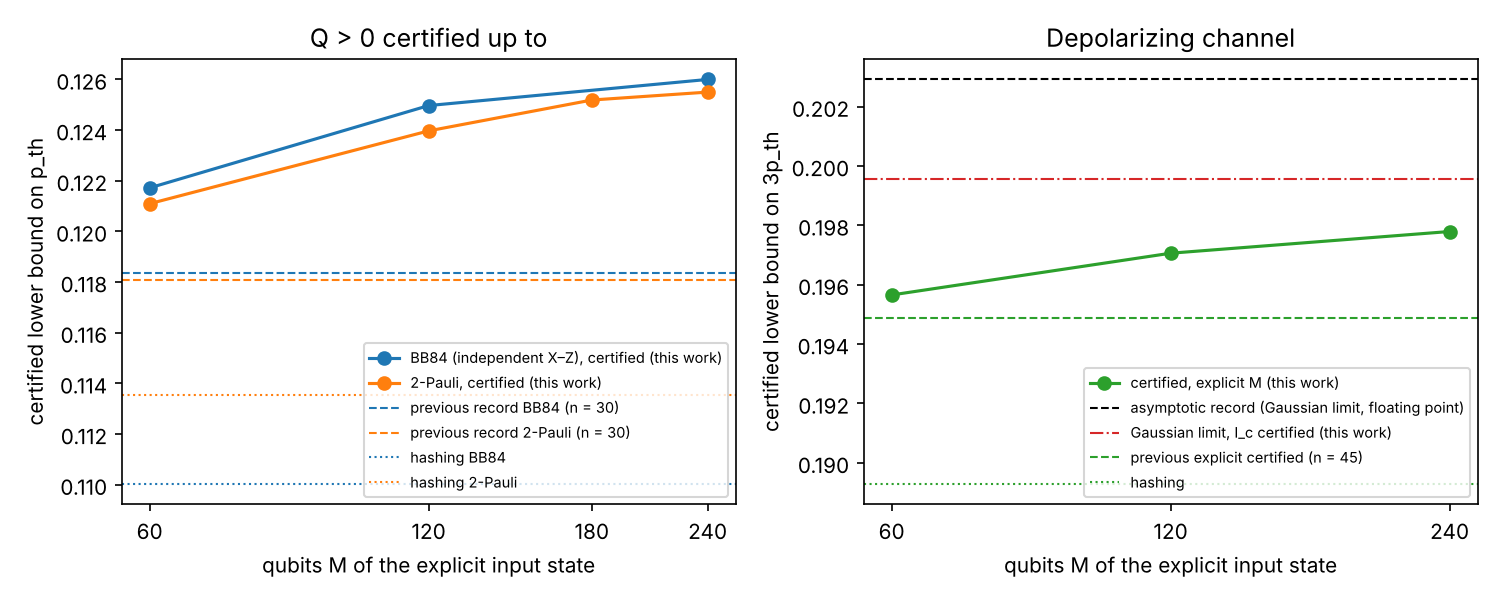
\includegraphics[width=\textwidth]{thresholds.png}
\caption{Certified lower bounds on $p_{\mathrm{th}}$ versus the number $M$ of qubits of the explicit input
state (best code per $M$, Table~\ref{tab:certs}). Left: BB84 and 2-Pauli; dashed, the previously reported
values at $n=30$~\cite{agarwal2026symmetry}; dotted, hashing. Right: depolarizing channel in total error
$3p$; black dashed, the asymptotic Gaussian-limit value $0.2029161$~\cite{ahmed2026choir} (floating point);
red dash-dotted, our certified Gaussian-limit value $0.1997875$ (Sec.~\ref{sec:depgauss}); green dashed,
the previous certified explicit value $0.194868$ ($n=45$)~\cite{krohn2026certified}; dotted, hashing.}
\label{fig:thresholds}
\end{figure*}

\paragraph*{Headline numbers.} $p_{\mathrm{th}}(\text{BB84})\ge0.126$ ($M=240$),
$p_{\mathrm{th}}(\text{2-Pauli})\ge0.1255$ ($M=240$), and, for the depolarizing channel, a certified
explicit-size value $3p=0.1977936$ ($M=240$). The last exceeds the previous explicit certified
$0.194868$ ($n=45$)~\cite{krohn2026certified} but not the asymptotic $0.2029161$~\cite{ahmed2026choir};
in the Gaussian limit we certify $0.1997875$ (Sec.~\ref{sec:depgauss}).
The BB84 and depolarizing families are closed under composition, with the less noisy channel as a
factor, so $Q>0$ also at every smaller noise. The 2-Pauli family is not ($XZ$ errors appear), so there
$p_{\mathrm{th}}\ge0.1255$ holds in the sup sense only.

\paragraph*{Codes.} For BB84 and 2-Pauli, mod-3 residue codes beat parity codes at the same $M$; for the
depolarizing channel we used mod-3 codes throughout, as in Ref.~\cite{ahmed2026choir}. The
sequence $M=30\to60\to120$ (BB84 $0.1185\to0.1217\to0.1239$, 2-Pauli $0.1180\to0.1211\to0.1232$, parity
codes) still rises with roughly geometric increments. The depolarizing explicit-$M$ values saturate:
$0.06522$, $0.06547$, $0.06569$ per Pauli at $M=60$, $90$, $120$, well below the asymptotic $0.06764$.
These sequences are bisection values, certified only where listed in Table~\ref{tab:certs}.

\subsection{A family between 2-Pauli and depolarizing}
\label{sec:family}
Let $(p_X,p_Y,p_Z)=p\,(1,1,r)/(2+r)$ with total error $p$ and the pole on $z$. $r=0$ is the 2-Pauli
channel with $p=2p_{\mathrm{2P}}$ (up to relabeling), and $r=1$ is the depolarizing channel with $p=3p_{\mathrm{dep}}$.
Table~\ref{tab:family} lists the certified points. The gain over hashing is $0.006$--$0.023$ across the
family, and the certified thresholds decrease monotonically from 2-Pauli to depolarizing. We found no
point-by-point records for the interior of this family in the literature. Bausch and
Leditzky~\cite{bausch2021pauli} cover the Pauli simplex with graph-state codes; we did not compare point
by point.

\begin{table}[t]
\caption{Family $r$: hashing point and certified thresholds (total error $p$; mod-3 codes; certifier B
unless noted).}
\label{tab:family}
\begin{ruledtabular}
\begin{tabular}{llll}
$r$ & hashing & certified, $M=60$ & certified, larger $M$\\
\hline
0 & 0.227092 & 0.2421876 (parity) & 0.2479376 ($M=120$)\\
1/4 & 0.199895 & 0.2228375 & \\
1/2 & 0.192599 & 0.2099375 & \\
3/4 & 0.189926 & 0.2015875 & \\
1 & 0.189290 & 0.1956561 & 0.1977936 ($M=240$)\\
\end{tabular}
\end{ruledtabular}
\end{table}

\subsection{Gaussian limit of the depolarizing channel}
\label{sec:depgauss}
We continued the $M=240$ mod-3 code in the Gaussian limit (the thermal attenuator with $\nu=1/(2\eta)$)
with $\Ic$ and its gradient evaluated in 128-bit ball arithmetic (refined eigenbases, so that line searches
are not limited by the $\sim3\times10^{-14}$ noise floor of double precision for this problem), at
$N_{\mathrm{in}}=240$, $D=360$. At $\eta=2351/3200$, i.e.\ $p=849/12800$ per Pauli
($3p=0.198984375$; $T=5527201/8881600$, $G=5551/4702$), the code has certified
$\Ic\in[1.82651528,1.85766717]\times10^{-8}$ bits (certifier~L, flag masses $\sim10^{-56}$); at
$\eta=2939/4000$ ($3p=0.1989375$), $[1.07683723,1.07994494]\times10^{-7}$. An independent
re-implementation (pure loss then amplifier, the thermal master equation, and a beam splitter with a
Fock-mixed thermal environment; output cutoff 420 photons) gives $1.8455798\times10^{-8}$ and
$1.0787368\times10^{-7}$, with the routes agreeing to $10^{-13}$. With Theorem~6 of
Ref.~\cite{ahmed2026choir} (proved for the depolarizing channel), $p_{\mathrm{th}}\ge0.198984375$ in total
error, for sufficiently large $M$. The branch ends there for a genuine reason: at $\eta=0.734625$ the
optimized value is $\Ic=-1.3\times10^{-7}$, far above any rounding error, with the mean photon number
still near $20$.

More photons move the threshold. Stretching that state by a factor 2 in the residue index ($n=3m+r$,
$m\to2m$; mean photon number $38.5$) and optimizing at $\eta=3673/5000$, where the 20-photon branch is
negative, gives $p=1327/20000$ per Pauli ($3p=0.19905$; $T=13490929/21682500$, $G=8673/7346$) with
certified $\Ic\in[1.52256332,1.54665840]\times10^{-8}$ bits; the independent re-implementation gives
$1.5376335\times10^{-8}$. Continuing this branch, the mean photon number stays at $38.5$ while $\Ic$
keeps growing under further optimization; at $\eta=7341/10000$, i.e.\ $p=2659/40000$ per Pauli
($3p=0.199425$; $T=53890281/86705000$, $G=17341/14682$), the code has certified
$\Ic\in[4.69714037,4.72320460]\times10^{-8}$ bits (independent re-implementation: $4.7133075\times10^{-8}$; intermediate certified points: $3p=0.1992375$ and
$0.19933125$; at $\eta=0.7335$, $60$ L-BFGS steps still leave $\Ic=-8.6\times10^{-8}$). Stretching once more (by $1.5$, mean photon number $57.5$) gives a branch that is positive at
$\eta=11743/16000$, i.e.\ $p=4257/64000$ per Pauli ($3p=0.199546875$; $T=137898049/221944000$,
$G=27743/23486$): certified $\Ic\in[2.57112611,2.97906949]\times10^{-9}$ bits, independent value
$2.8369733\times10^{-9}$. Continuing it, the lowest certified point is $\eta=3756117/5120000$, i.e.\
$p=1363883/20480000$ per Pauli ($3p=0.199787548828125$; $T=14108414917689/22722859520000$,
$G=8876117/7512234$), with $\Ic\in[4.99212570,8.85924622]\times10^{-10}$ bits (independent value
$7.472121\times10^{-10}$); points that failed once
passed on a later visit from a better state, so the branch is limited by the optimization budget (we
stopped at $\sim2\times10^{-5}$ in $3p$ per 12-minute step). Hence $p_{\mathrm{th}}\ge0.1997875$ with Theorem~6 of
Ref.~\cite{ahmed2026choir}. The gain per stretch shrinks ($\eta\approx0.73467$, $0.7341$, $0.7337$ for
$20$, $38.5$, $57.5$ photons), so stretching alone does not reach $\eta=0.7294452$: the $56$-photon record
code must have a different structure.
The coherent information shrinks as the photon number grows, which is the trade-off that leads to the
$56$-photon codes of the floating-point record.

\subsection{Gaussian limit of the 2-Pauli channel}
For the emergent 2-Pauli channel at $p=31/250=0.124$ ($T=94/125$, $G=94/63$), a mod-4 residue code with
codewords on $n\equiv0,2\pmod4$ ($N_{\mathrm{in}}=160$, $D=280$, flag mass $2\times10^{-17}$) has
certified $\Ic\in[1.96141999,1.96142031]\times10^{-4}$ bits (certifier~L). Transferring this to the qubit
channel would require extending the convergence theorem of Ref.~\cite{ahmed2026choir} to the 2-Pauli
channel. The explicit $M=180$ certificate ($0.1251875$) makes that step unnecessary for the record.

% =====================================================================================================
\section{The additive Gaussian noise channel beyond $\sigma^2=1/e$}
\label{sec:agn}

By Eq.~\eqref{eq:sigmaq}, the Gaussian limit of the BB84 channel is the AGN channel
$\Nsig$: $V\mapsto V+\sigma^2\one$, $X=\one$. It agrees with the Gaussian random displacement channel of
Ref.~\cite{lin2025gkp} ($\hat q=(a+a^\dagger)/\sqrt2$, covariance shifted by $\sigma^2\one$).
Moreover,
\begin{equation}
  \Nsig=\Amp_G\circ\Loss_T,\qquad G=1+\sigma^2,\quad T=1/G,
  \label{eq:agnTG}
\end{equation}
since both sides are Gaussian with $X=\sqrt{GT}\,\one=\one$ and
$Y=\frac{G(1-T)}2+\frac{G-1}2=G-1=\sigma^2$. Since $\mathcal N_{\sigma_2}\circ\mathcal N_{\sigma_1}=
\mathcal N_{\sqrt{\sigma_1^2+\sigma_2^2}}$, data processing makes $Q(\Nsig)$ nonincreasing in $\sigma$.

Known bounds (Sec.~\ref{sec:intro}): $Q(\Nsig)>0$ for $\sigma^2<1/e$ (thermal
inputs~\cite{holevo2001evaluating}, GKP codes~\cite{harrington2001achievable}) and $Q(\Nsig)=0$ for
$\sigma^2\ge\frac12$~\cite{caruso2006degradability,lami2019extendibility}. Explicit GKP codes with
maximum-likelihood decoding reach $\sigma=0.598$~\cite{lin2025gkp}.

\begin{theorem}[computer-assisted]
\label{thm:agn}
Let $\rho=(\ket{\phi_0}\bra{\phi_0}+\ket{\phi_1}\bra{\phi_1})/Z$, where the real amplitudes of
$\phi_0$ (supported on $n\equiv0\pmod3$) and $\phi_1$ (on $n\equiv1\pmod3$), $n\le140$, are the float64
numbers stored in the file \texttt{agn\_k3\_sigma2\_0.4.npy} (sha256 \texttt{7917b7de2ccf2add}\dots;
Sec.~\ref{sec:repro}). At
$\sigma^2=2/5$,
\begin{equation}
  \Ic(\rho,\mathcal T_{320}\circ\Nsig)\in[3.35715244,\ 3.35738269]\times10^{-6}\ \text{bits}.
\end{equation}
Consequently $Q(\Nsig)\ge3.357\times10^{-6}$ qubits per channel use at $\sigma^2=2/5$. Likewise, the
mod-3 state stored in \texttt{agn\_k3\_sigma2\_0.405.npy} (sha256 \texttt{7e39e6ffc2144ccc}\dots,
$n\le300$) satisfies, at $\sigma^2=81/200$,
\begin{equation}
  \Ic(\rho',\mathcal T_{600}\circ\Nsig)\in[6.33597116,\ 6.40767279]\times10^{-8}\ \text{bits},
\end{equation}
so $Q(\Nsig)>0$ for every $\sigma^2\le81/200$. Finally, the rank-two input $\rho''$ without residue
structure stored in \texttt{agn\_gen\_sigma2\_0.407.npy} (sha256 \texttt{cb6c059e736810ac}\dots, $n\le200$)
satisfies, at $\sigma^2=407/1000$,
\begin{equation}
  \Ic(\rho'',\mathcal T_{400}\circ\Nsig)\in[5.43799903,\ 5.50010769]\times10^{-8}\ \text{bits},
\end{equation}
and its continuation $\rho'''$ (\texttt{agn\_gen\_sigma2\_0.4075.npy}, sha256 \texttt{756c07a44641776b}\dots,
$n\le300$) satisfies, at $\sigma^2=163/400$,
\begin{equation}
  \Ic(\rho''',\mathcal T_{600}\circ\Nsig)\in[5.97733793,\ 6.88032591]\times10^{-9}\ \text{bits},
\end{equation}
so $Q(\Nsig)>0$ for every $\sigma^2\le163/400$. Finally, the mod-3 state $\rho''''$ obtained by stretching
$\rho'$ to a mean photon number of $29.3$ (\texttt{agn\_k3s2\_sigma2\_0.4111875.npy}, sha256
\texttt{c7b1356a3fdff992}\dots, $n\le300$) satisfies, at $\sigma^2=6579/16000$,
\begin{equation}
  \Ic(\rho'''',\mathcal T_{600}\circ\Nsig)\in[9.61014601,\ 13.2820991]\times10^{-10}\ \text{bits},
\end{equation}
so $Q(\Nsig)>0$ for every $\sigma^2\le6579/16000=0.4111875$, i.e.\ $\sigma\le0.6412$.
\end{theorem}

\begin{proof}[Certificate]
Certifier~L (Sec.~\ref{sec:certify}) with the exact decomposition~\eqref{eq:agnTG}, $G=7/5$, $T=5/7$,
$N_{\mathrm{in}}=140$ and $D=320$. The flag masses are $3.4\times10^{-47}$ and $3.9\times10^{-47}$, and
the widths of the entropy enclosures are below $6\times10^{-11}$ nats per residue block. The
consequences follow from data processing (Sec.~\ref{sec:certify}) and the monotonicity in $\sigma$.
\end{proof}

\paragraph*{The code.} The two codewords carry weights $0.446$ and $0.554$, and the state has mean photon
number $15.4$. It was obtained by transferring the $M=240$ BB84 mod-3 code (Table~\ref{tab:certs},
excitations $k\mapsto$ Fock $n$) to the emergent channel and re-optimizing it by continuation in $q$.
That optimization ran in floating point up to $q=0.1279375$ ($\sigma^2\approx0.40298$), and the
resulting state was certified, without further changes, at the slightly smaller noise $\sigma^2=2/5$.
The truncation is generous: the same certificate also passes with $D=380$. A re-run of the
certifier with single-threaded BLAS gave the nested interval $[3.35715258,3.35738262]\times10^{-6}$.
The enclosure endpoints depend on the floating-point approximate eigenbasis, and every such interval is
rigorous.

\paragraph*{Independent check.} A separate AI-agent instance, without importing any repository code,
implemented the channel as the diffusion semigroup $\exp[\sigma^2(\mathcal D[a]+\mathcal D[a^\dagger])]$.
It checked that this adds exactly $\sigma^2$ to both quadrature variances and maps the vacuum to a
thermal state with $\bar n=\sigma^2$. It cross-checked the Fock matrix elements four ways to $10^{-15}$
(high-precision quadrature of the displacement average, the Lindblad propagator, $\Amp_G\circ\Loss_T$
and $\Loss_{T'}\circ\Amp_{G'}$), and obtained $\Ic=3.3572969\times10^{-6}$ bits for the stored state at
$\sigma^2=2/5$, stable for cutoffs 320, 400 and 520 and inside the certified interval. Its values also
agree with ours at $\sigma^2=0.38$, $0.403$, $0.404$ and $0.405$; at $0.405$ the coherent information of
this state is negative. For the second state it obtained $\Ic=6.38363\times10^{-8}$ bits at
$\sigma^2=81/200$ (cutoffs 600, 700 and 800 agree to $3\times10^{-13}$), inside the certified interval,
and reproduced the certificate exactly; the coherent information of that state changes sign at
$\sigma^2\approx0.40509$. This is a floating-point re-computation, not a second rigorous certificate.

\paragraph*{How far it goes.} Re-optimizing the mod-3 family with a larger cutoff ($N_{\mathrm{in}}=300$,
$D=600$) gave the second state of Theorem~\ref{thm:agn} (mean photon number $15.4$), certified at
$\sigma^2=81/200$ with flag masses below $6\times10^{-56}$; in floating point its coherent information is
$1.08\times10^{-6}$ at $\sigma^2=0.4035$ and $6.4\times10^{-8}$ at $0.405$. Other residue families with the same cutoff stop earlier in floating point
(coherent information above $10^{-6}$ required): mod~4 $\{0,2\}$ (about 72 photons) at $0.40175$, parity
and mod~5 $\{0,1\}$ at $0.39975$, mod~5 $\{0,2\}$ at $0.39575$, mod~4 $\{0,1\}$ at $0.39375$ and mod~6
$\{0,3\}$ at $0.39175$. Rank-three mod-3 inputs do not help: the optimum stays of rank two.

\paragraph*{Breaking the symmetry.} Optimizing over all rank-two inputs ($N_{\mathrm{in}}=200$, $D=400$),
starting from the mod-3 state plus a small random perturbation, gives states that remain about $99.9\%$ on
the residues but carry about $0.1\%$ of weight off them in each codeword (overlap
$\langle\phi_0|\phi_1\rangle\approx-7\times10^{-4}$). This small breaking of the $\mathbb Z_3$ symmetry
multiplies the coherent information: $4.37\times10^{-7}$ instead of $6.4\times10^{-8}$ at $\sigma^2=0.405$
(certified: $[4.36362113,4.37080935]\times10^{-7}$ bits), and continuation in $\sigma^2$ keeps it positive up
to $0.407$ (third certificate) and, with $N_{\mathrm{in}}=300$ and $D=600$, to $0.4075$ (fourth certificate);
it is negative at $0.408$. Starting instead from the high-energy mod-4 $\{0,2\}$ state (about 77 photons)
with broken symmetry stops at $0.406$. Without residue structure
the output of $\mathrm R\otimes\mathrm B$ is certified as a single $802\times802$ block, and the flag block
of $\mathrm R\otimes\mathrm B$ is no longer diagonal: its entropy is enclosed by $[h(t),h(t)+t\ln2]$, with
$t$ the total flag mass ($\approx7\times10^{-44}$), which holds for any $2\times2$ positive matrix of
trace $t$. So the residue codes are not local maxima in the full input space, and the true threshold of
single-mode rank-two inputs is somewhat above what residue families suggest. The optimal codewords
are not three-component cat codes, which give $\Ic<10^{-12}$ for every $\sigma^2\in[0.36,0.39]$ after
optimizing the amplitude and weights; they have a positive main lobe at $n\approx3$--$18$ and a tail of
alternating sign, with photon-number variance about $2.7$ times the Poisson value. A three-parameter physical family explains most of the
gain: \emph{squeezed cats}, the $n\equiv0$ and $n\equiv1\pmod3$ parts of a displaced phase-squeezed state
$D(\alpha)S(r)\ket0$ with weights $w,1-w$. With $\alpha\approx5.71$, $r\approx-1.03$, $w\approx0.452$ it is positive
up to $\sigma^2=0.392$; at $\sigma^2=49/125$ (file \texttt{agn\_sqcat\_sigma2\_0.392.npy}, sha256
\texttt{eb13a99ef8255ad0}\dots) we certify $\Ic\in[1.73865751,1.73880842]\times10^{-6}$ bits. So more than half ($56\%$) of
the improvement over $1/e$ comes from a state of a kind already prepared in optical experiments. The independent
re-implementation, with full matrices and two different purifications, gives $4.3682405\times10^{-7}$ and
$5.4779650\times10^{-8}$ bits for the two symmetry-free states, and $6.58088\times10^{-9}$ bits (three routes) for
the fourth, all inside the certified intervals.

\paragraph*{More photons.} The trick that moved the depolarizing branch (Sec.~\ref{sec:depgauss}) also
works here. Stretching the mod-3 state $\rho'$ ($15.4$ photons) in the residue index ($n=3m+r$,
$m\to\lambda m$, amplitudes interpolated) by $\lambda=1.5$ and $2$ gives mean photon numbers $22.1$ and $29.3$,
and continuation in $\sigma^2$ keeps both positive well beyond the symmetry-free states: the $22$-photon
code is certified at $\sigma^2=51/125$ ($[9.57696812,9.62308372]\times10^{-8}$ bits) and $41/100$
($[1.85979392,1.92549153]\times10^{-8}$), and the $29$-photon code, which overtakes it near $0.411$, at
$411/1000$ ($[1.17506701,1.58865651]\times10^{-9}$), $3289/8000$ and $6579/16000$ (Theorem~\ref{thm:agn}).
At $\sigma^2=0.4075$ the $22$-photon code has $\Ic=1.25\times10^{-7}$, twenty times the symmetry-free state.
As for the depolarizing channel, more photons give a higher threshold with a smaller margin, and the
optimization budget, not the code, sets the last digits (a longer optimization at $0.4115$ climbs from
$-2.5\times10^{-9}$ to $-2\times10^{-12}$). The independent re-implementation (five routes: loss then
amplifier, amplifier then loss, the diffusion semigroup by uniformization and by dense exponentiation,
and unitary dilations; cutoffs 600--800) gives $9.6074153\times10^{-8}$, $1.9038668\times10^{-8}$,
$1.4606876\times10^{-9}$, $1.2823360\times10^{-9}$ and $1.2180839\times10^{-9}$ bits for the five
certified points, all inside the intervals, with the routes agreeing to $10^{-13}$.
The interval $0.4111875<\sigma^2<1/2$ remains open.

\paragraph*{Consequences.} At $\sigma^2=2/5$ the coherent information optimized over Gaussian inputs is
zero, while $Q(\Nsig)\ge3.357\times10^{-6}$. Hence the Gaussian-optimized one-shot coherent
information is not the quantum capacity of the additive Gaussian noise channel, which settles in the
negative the speculation of Harrington and Preskill quoted in Sec.~\ref{sec:intro}, and the
one-shot coherent information itself is strictly larger than its Gaussian restriction there. To our
knowledge this is the first rigorous proof of $Q(\Nsig)>0$ for any $\sigma>1/\sqrt e$; the
simulation-based threshold $\sigma\approx0.67$ of Ref.~\cite{zhang2023xzzx}, if confirmed, would go further.

\paragraph*{Relation to the thermal attenuator.} Write $\mathcal E_{\eta,\nu}$ for the thermal attenuator
with transmissivity $\eta$ and $\nu$ thermal photons, $Y=(1-\eta)(\nu+\frac12)$. Two exact Gaussian
identities connect it to $\Nsig$:
\begin{equation}
\begin{aligned}
  \mathcal E_{\eta,\nu}&=\Loss_\eta\circ\mathcal N_{\sigma'}, & \sigma'^2&=(1-\eta)\nu/\eta,\\
  \Amp_{1/\eta}\circ\mathcal E_{\eta,\nu}&=\mathcal N_{\sigma''}, & \sigma''^2&=(1-\eta)(\nu+1)/\eta.
\end{aligned}
  \label{eq:thermalrel}
\end{equation}
The first identity shows that the result of Mele \textit{et al.}~\cite{mele2026thermal} implies
positivity for $\mathcal N_{\sigma'}$ only. At their point $\nu=1$, $\eta=0.7841$ this is
$\sigma'^2=0.275<1/e$, so it does not imply Theorem~\ref{thm:agn}. Conversely, the second identity and
Theorem~\ref{thm:agn} give $Q(\mathcal E_{\eta,\nu})>0$ whenever $(1-\eta)(\nu+1)/\eta\le0.4111875$. For
$\nu>3.84$ this region extends below the Holevo--Werner thermal-state threshold
$\log_2\frac{\eta}{1-\eta}=g(\nu)$, with $g(\nu)=(\nu+1)\log_2(\nu+1)-\nu\log_2\nu$; for example, at
$\nu=10$ it covers $\eta\in[0.96397,0.96614)$. We have not compared this with the non-Gaussian results of
Ref.~\cite{mele2026thermal} away from $\nu=1$.
The same argument applies to the thermal amplifier $\mathcal A_{\tau,\nu}$ ($X=\sqrt\tau\,\mathbb 1$,
$Y=(\tau-1)(\nu+\frac12)\mathbb 1$, $\tau>1$): $\Loss_{1/\tau}\circ\mathcal A_{\tau,\nu}=\mathcal N_{\sigma'''}$ with
$\sigma'''^2=(\tau-1)(\nu+1)/\tau$, so $Q(\mathcal A_{\tau,\nu})>0$ whenever $(\tau-1)(\nu+1)/\tau\le0.4111875$. In
general, a phase-insensitive channel with transmissivity or gain $\tau$ and added noise $Y$ has $Q>0$
whenever $(Y+|1-\tau|/2)/\tau\le0.4111875$. For both families the new region lies beyond the Gaussian-input
threshold exactly when $2^{g(\nu)}>(\nu+1)/0.4111875$, i.e.\ for $\nu>3.84$; at $\nu=10$ the amplifier
window is $\tau\in(1.03632,1.03883]$.

\paragraph*{A thermal amplifier at low noise.} The emergent channel of the 2-Pauli family,
$\Amp_G\circ\Loss_T$ with $T=1-2p$ and $G=(1-2p)/(1-4p)$, is a thermal amplifier, and the corollary above
does not reach the relevant parameters. The mod-3 code transferred from $M=240$ and continued in the
Gaussian limit to $p=0.12725$ (file \texttt{amp\_2p3\_p0.1275.npy}, sha256 \texttt{57ba63a1717f0653}\dots)
gives, at $p=51/400$, i.e.\ $T=149/200$ and $G=149/98$,
\begin{equation}
  \Ic\in[9.10836870,\ 9.11017611]\times10^{-7}\ \text{bits}.
\end{equation}
This channel is the thermal amplifier with gain $\tau=22201/19600\approx1.1327$ and $\nu=149/51\approx2.922$
thermal photons. At this gain thermal inputs give positive coherent information only for $\nu<2.6533$
($\log_2\frac{\tau}{\tau-1}-g(\nu)=-0.1187$ at $\nu=149/51$), and the channel is antidegradable only for
$\nu\ge3.768$ ($Y\ge\tau/2$). Its additive-noise equivalent has $\sigma^2=0.459>0.4111875$, so this is not a
consequence of Theorem~\ref{thm:agn}. We know of no earlier non-Gaussian positivity result for thermal
amplifiers. The same independent re-implementation (three routes: the Lindblad semigroup with gain and loss
rates, $\Loss_{T'}\circ\Amp_{G'}$, and $\Amp_G\circ\Loss_T$) gives $\Ic=9.109425\times10^{-7}$ bits, inside
the interval, and a sweep of thermal and squeezed-thermal inputs in 60-digit arithmetic found no Gaussian
input with positive coherent information. Breaking the residue symmetry, as for the AGN channel, a
rank-two input stays positive up to $p=0.128$ and is certified at $p=16/125$ ($T=93/125$, $G=93/61$, i.e.\
$\tau=8649/7625\approx1.1343$ and $\nu=93/32\approx2.906$): $\Ic\in[1.43395294,1.43876228]\times10^{-7}$ bits,
where thermal inputs need $\nu<2.6206$ and antidegradability starts at $\nu=3.7231$. The independent re-implementation gives
$1.4369750\times10^{-7}$ bits for this state, inside the interval.

\paragraph*{The thermal attenuator with one thermal photon.} For $\mathcal E_{\eta,\nu}$ with $\nu=1$, Mele
\textit{et al.}~\cite{mele2026thermal} certified $Q>0$ down to $\eta=0.7841$ (thermal inputs stop at
$\eta=0.8$, antidegradability starts at $\eta=0.75$; their uncertified numerics suggest $\eta\approx0.7818$).
Our optimizer and certifier apply directly, with $\mathcal E_{\eta,\nu}=\Amp_G\circ\Loss_T$,
$G=(1-\eta)(\nu+\frac12)+\frac{1+\eta}2$, $T=\eta/G$. Among residue families at low energy, mod~3 $\{0,1\}$
is best (about 17 photons; parity stops at $\eta=0.78525$, mod~4 $\{0,1\}$ at $0.78375$). At
$\eta=3133/4000=0.78325$ (file \texttt{th1\_k3\_p0.21675.npy}, sha256 \texttt{eff871b4adcf91ce}\dots,
$N_{\mathrm{in}}=80$, $D=240$),
\begin{equation}
  \Ic\in[8.27408111,\ 8.27425105]\times10^{-6}\ \text{bits}.
\end{equation}
Since $\mathcal E_{\eta,\nu}=\mathcal E_{\eta/\eta',\nu}\circ\mathcal E_{\eta',\nu}$, $Q$ is non-decreasing in
$\eta$, so $Q(\mathcal E_{\eta,1})>0$ for all $\eta\ge0.78325$, improving the certified value $0.7841$. The
independent re-implementation, starting from the beam-splitter definition with a thermal environment of
mean photon number $\nu$ (as in Ref.~\cite{mele2026thermal}) and using four routes, gives
$\Ic=8.2742014\times10^{-6}$ bits, inside the interval; thermal and squeezed-thermal inputs are all
negative at this point. Breaking the residue symmetry goes further: a rank-two input stays positive to
$\eta=0.78$ (file \texttt{th1\_gen\_eta0.78.npy}, sha256 \texttt{6c91dfe91ec43e9f}\dots, $N_{\mathrm{in}}=120$,
$D=300$), where $\Ic\in[2.12631890,2.16095917]\times10^{-8}$ bits; the independent re-implementation gives
$2.150005\times10^{-8}$. Hence $Q(\mathcal E_{\eta,1})>0$ for all $\eta\ge0.78$, below both the certified
$0.7841$ and the uncertified numerical $0.7818$ of Ref.~\cite{mele2026thermal}; the window
$0.75<\eta<0.78$ remains open.

\paragraph*{All temperatures.} Ref.~\cite{mele2026thermal} treats $\nu=1$ only. The same codes certify $Q>0$
inside the open window $(\eta_{\mathrm{AD}},\eta_{\mathrm G})$, with $\eta_{\mathrm{AD}}=(\nu+\frac12)/(\nu+1)$
and $\eta_{\mathrm G}=2^{g(\nu)}/(1+2^{g(\nu)})$, at every $\nu$ we tried (Table~\ref{tab:nu} and
Fig.~\ref{fig:numap}); for $\nu\gtrsim4.2$ the AGN corollary also applies but the direct certificates go
further. Since $Q$ is monotone in $\eta$ at fixed $\nu$, each row certifies $Q>0$ for all larger $\eta$. The independent re-implementation (three routes per point) gives values inside every interval of
Table~\ref{tab:nu}, and it regenerated the squeezed-cat state from $(\alpha,r,w)$ to $4\times10^{-16}$.

\begin{table*}[t]
\caption{Thermal attenuator with $\nu$ thermal photons: certified $Q>0$ at transmissivity $\eta$, with the
fraction of the open window $(\eta_{\mathrm{AD}},\eta_{\mathrm G})$ it closes. Inputs are rank two,
symmetry-free ($k=1$, $N_{\mathrm{in}}=160$, $D=360$) except $\nu=5$ (mod~3, $N_{\mathrm{in}}=260$, $D=520$) and $\nu=1$ ($N_{\mathrm{in}}=120$,
$D=300$).}
\label{tab:nu}
\begin{ruledtabular}
\begin{tabular}{lllll}
$\nu$ & $\eta_{\mathrm{AD}}$ & $\eta_{\mathrm G}$ & certified $\eta$ & $\Ic$ (bits)\\
\hline
1/4 & 0.6 & 0.65147 & 313/500 (50\%) & $[2.48378509,2.48746745]\times10^{-7}$\\
1/2 & 0.66667 & 0.72207 & 1393/2000 (46\%) & $[6.31451396,6.36306427]\times10^{-8}$\\
1 & 0.75 & 0.8 & 39/50 (40\%) & $[2.12631890,2.16095917]\times10^{-8}$\\
2 & 0.83333 & 0.87097 & 8587/10000 (33\%) & $[1.14709176,1.14892934]\times10^{-7}$\\
3 & 0.875 & 0.90459 & 1791/2000 (31\%) & $[8.31897855,8.33853440]\times10^{-8}$\\
5 & 0.91667 & 0.93723 & 7459/8000 (24\%) & $[1.17390097,1.17400578]\times10^{-6}$\\
\end{tabular}
\end{ruledtabular}
\end{table*}

\begin{figure*}[t]
\centering
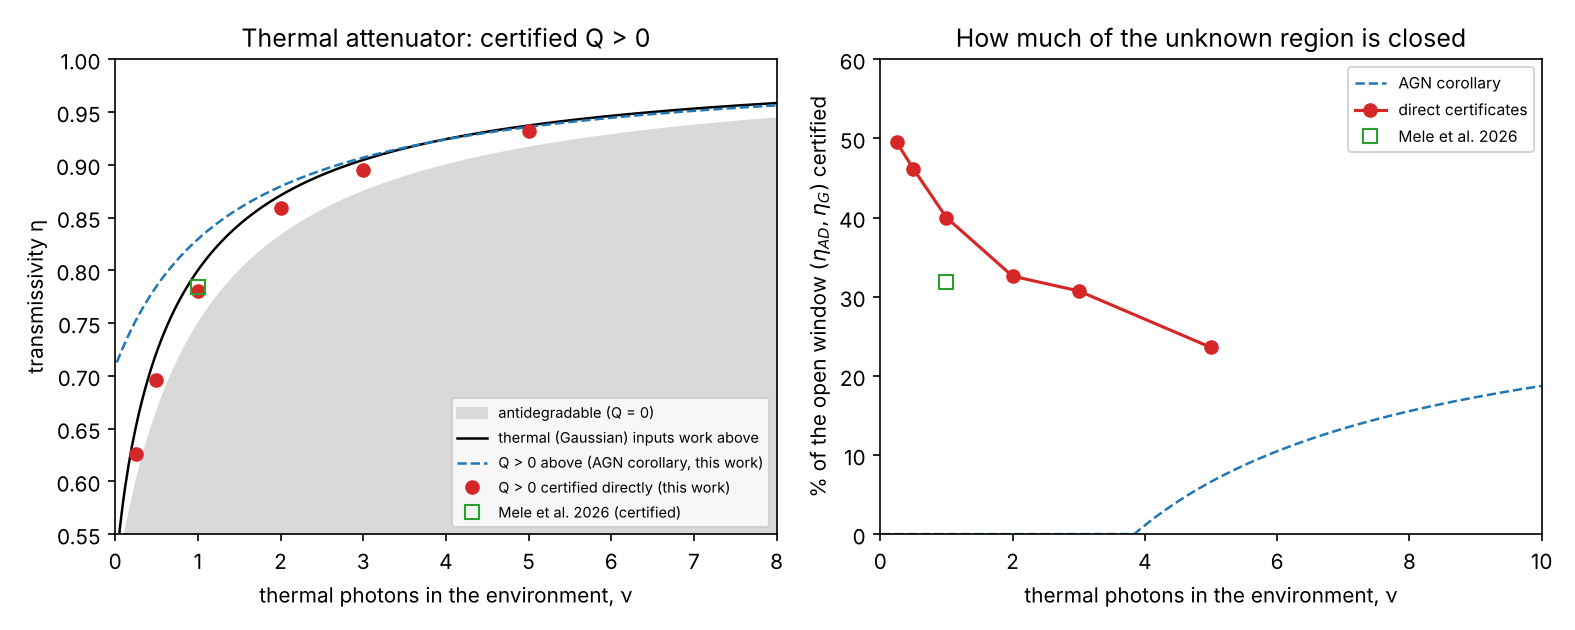
\includegraphics[width=\textwidth]{attenuator_map.png}
\caption{Thermal attenuator. Left: certified $Q>0$ above the red points (direct certificates) and above the
dashed curve (corollary of Theorem~\ref{thm:agn}); thermal inputs work above the solid curve; gray:
antidegradable. Right: fraction of the open window closed at each $\nu$; the square is the certified point of
Ref.~\cite{mele2026thermal}.}
\label{fig:numap}
\end{figure*}

\begin{figure}[t]
\centering
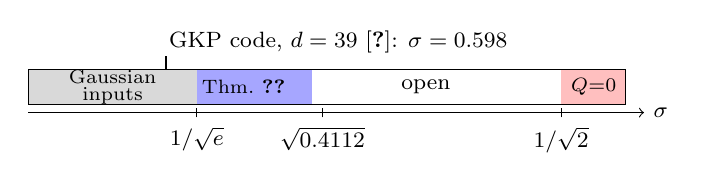
\begin{tikzpicture}[x=46cm,y=1cm,font=\footnotesize]
  \fill[gray!30] (0.56,0) rectangle (0.60653,0.45);
  \fill[blue!35] (0.60653,0) rectangle (0.63836,0.45);
  \fill[red!25] (0.70711,0) rectangle (0.725,0.45);
  \draw (0.56,0) rectangle (0.725,0.45);
  \node[font=\scriptsize,align=center] at (0.5833,0.225) {Gaussian\\[-2pt]inputs};
  \node[font=\scriptsize] at (0.6195,0.225) {Thm.~\ref{thm:agn}};
  \node at (0.6698,0.225) {open};
  \node[font=\scriptsize] at (0.7161,0.225) {$Q{=}0$};
  \draw[->] (0.56,-0.1) -- (0.73,-0.1) node[right] {$\sigma$};
  \foreach \s/\l in {0.60653/{$1/\sqrt e$}, 0.64124/{$\sqrt{0.4112}$}, 0.70711/{$1/\sqrt2$}} {
    \draw (\s,-0.16) -- (\s,-0.04);
    \node[below] at (\s,-0.16) {\l};
  }
  \draw[thick] (0.598,0.45) -- (0.598,0.62);
  \node[above right,inner sep=1pt] at (0.598,0.62) {GKP code, $d=39$~\cite{lin2025gkp}: $\sigma=0.598$};
\end{tikzpicture}
\caption{Positivity of $Q(\Nsig)$ along $\sigma$. Gray: thermal inputs~\cite{holevo2001evaluating};
blue: this work (Theorem~\ref{thm:agn}); white: open; red: antidegradable. The bar marks the largest
$\sigma$ with a nonzero rate for an explicit GKP code reported in Ref.~\cite{lin2025gkp}.}
\label{fig:agn}
\end{figure}

% =====================================================================================================
\section{What did not work}
\label{sec:failures}

\paragraph*{The depolarizing record.} We did not beat $3p=0.2029161$; our certified Gaussian-limit value
is $0.1997875$ (Sec.~\ref{sec:depgauss}), and the symmetry breaking that
helps for the AGN channel did not help here. Full L-BFGS over residue codes
($\kappa=2,\dots,6$, ranks 2--3) for the emergent thermal attenuator, in float64, reaches $\Ic>0$ only
down to $\eta\approx0.737$ ($3p\approx0.197$). The record point $\eta=0.7294452$ needs codes with mean
photon number $\approx56$~\cite{ahmed2026choir}. In that regime the three phase components are almost
orthogonal both for Bob and for the environment, and $\Ic\approx0$ with curvature $\approx-0.16$ and
gradient $\sim10^{-6}$. Only $\sim10^{-11}$ of coherent information is available there, consistent with
the $10^{-12}$ reported in Ref.~\cite{ahmed2026choir}. In 128-bit arithmetic, mod-3 codes with Gaussian
envelopes are negative at $\eta=0.7294452$ for every mean photon number ($40$--$70$), width ($2$--$6$)
and weight ($0.30$--$0.62$) we scanned, with $|\Ic|$ between $10^{-5}$ and $10^{-28}$ (one is enclosed
rigorously as $-4.66625545720\times10^{-12}$), and they stay negative up to $\eta=0.75$; squeezed-cat
codes behave the same way. The record code therefore has structure beyond a Gaussian envelope that we
have not found, and without it we can neither confirm nor refute the floating-point value. Large-amplitude coherent-state cat codes do worse:
the quantum Chernoff overlap exponents of Bob and of the environment cross at $\eta=0.7757$. With
explicit $M$, the thresholds saturate (Sec.~\ref{sec:results}): reaching $56$ excitations needs $M$ far
beyond the $240$ used here.

\paragraph*{Strongly biased noise.} By Table~\ref{tab:bias}, the Gaussian route is useless for
dephasing-biased noise with $b\gtrsim1$, where the ceiling is below the hashing point.

\paragraph*{Float64 certification for 2-Pauli at large $M$.} Because $\mu_1$ grows with $M$, the float64
budget for 2-Pauli loses up to $e^{\mu_1}$, and the 2-Pauli entries at $M\ge180$ require extended
precision.

% =====================================================================================================
\section{Open problems}
\label{sec:open}
\begin{itemize}
\item Prove the Gaussian limit (the analogue of Theorem~6 of Ref.~\cite{ahmed2026choir}) for
phase-covariant Pauli channels, for instance along Remark~\ref{rem:mechanism}, and for general Pauli
channels with Eq.~\eqref{eq:XY}.
\item Find the optimal Gaussian-limit codes and turn them into finite-$M$ thresholds. The certified Gaussian-limit
values correspond to $q\approx0.1296$ for BB84 ($\sigma^2=0.4111875$) and $p=0.128$ for the 2-Pauli channel (the
thermal-amplifier certificate); a convergence theorem for these channels would make them thresholds of the
qubit channels. Multi-mode (degenerate) codes are unexplored here. The ceiling is $0.146447$.
\item Close the AGN window $0.4111875<\sigma^2<1/2$: is $Q(\Nsig)>0$ for every $\sigma^2<1/2$?
\item Push explicit $M$ further: thresholds still rise with $M$, and certifier~B scales like the float
computation itself.
\item Depolarizing: an explicit-$M$ certificate approaching $0.2029$ needs states with $\sim56$
excitations, i.e.\ $M$ in the thousands, or a quantitative convergence theorem.
\item An independent, dependency-free verifier in exact integer arithmetic, in the spirit of
Ref.~\cite{krohn2026certified}, and human verification of the present certificates.
\end{itemize}

% =====================================================================================================
\section{Reproducibility}
\label{sec:repro}

Code, input states and logs are in the accompanying repository~\cite{repo}, in
\texttt{pauli-emergence/} and \texttt{depolarizing-threshold/}. Requirements are Python 3
with \texttt{numpy}, \texttt{scipy}, \texttt{python-flint} (0.9.0 was used) and \texttt{qutip} (only for
cross-checks). The runs used Python~3.13, NumPy~2.5.3 and SciPy~1.18.1 on x86-64. The script
\texttt{recertify\_all.sh} runs certifier~B with \texttt{OMP\_NUM\_THREADS=1} and bands in parallel
(\texttt{CERT\_PROCS=4}). The arguments are channel,
exact $p$, state file, $M$, $\kappa$ and residues (B, F), or channel, parameter, state file, residues,
$\kappa$, $N_{\mathrm{in}}$ and $D$ (L):
\par\medskip\noindent\begin{minipage}{\columnwidth}
\small
\begin{verbatim}
cd pauli-emergence
python3 certify_finite.py bb84 304297/2500000 \
    runs/cert_bb_M60_thr.npy 60 2 0,1
python3 certify_big.py bb84 63/500 \
    runs/state_bb3_M240_q0.126.npy 240 3 0,1
python3 certify_big.py depol 41207/625000 \
    runs/state_dep_M240_thr.npy 240 3 0,1
CERT_LD=1 CERT_PROCS=4 python3 certify_big.py \
    2pauli 2003/16000 \
    runs/state_2p3_M180_thr.npy 180 3 0,1
python3 certify_limit.py agn 2/5 \
    runs/agn_k3_sigma2_0.4.npy 0,1 3 140 320
python3 certify_limit.py agn 81/200 \
    runs/agn_k3_sigma2_0.405.npy 0,1 3 300 600
python3 certify_limit.py agn 407/1000 \
    runs/agn_gen_sigma2_0.407.npy 0,0 1 200 400
python3 certify_limit.py agn 163/400 \
    runs/agn_gen_sigma2_0.4075.npy 0,0 1 300 600
python3 certify_limit.py agn 6579/16000 \
    runs/agn_k3s2_sigma2_0.4111875.npy 0,1 3 300 600
python3 certify_limit.py 2pauli 31/250 \
    runs/2p_k4_p0.124.npy 0,2 4 160 280
python3 certify_limit.py 2pauli 51/400 \
    runs/amp_2p3_p0.1275.npy 0,1 3 140 320
python3 certify_limit.py 2pauli 16/125 \
    runs/amp_gen_p0.128.npy 0,0 1 200 400
python3 certify_limit.py th1 867/4000 \
    runs/th1_k3_p0.21675.npy 0,1 3 80 240
python3 certify_limit.py th1 11/50 \
    runs/th1_gen_eta0.78.npy 0,0 1 120 300
python3 certify_limit.py agn 49/125 \
    runs/agn_sqcat_sigma2_0.392.npy 0,1 3 140 320
# nu = 1/4, 1/2, 2, 3, 5: see CERTIFICATES.md
\end{verbatim}
\end{minipage}
\par\medskip
{\raggedright The full list of commands, state files and hashes is in \texttt{CERTIFICATES.md}, and
\texttt{recertify\_all.sh} re-runs all certifier-B entries. State files for the rows of
Table~\ref{tab:certs}, in order: \texttt{cert\_2p\_M60\_p0.1210938.npy}, \texttt{cert\_bb\_M60\_thr.npy},
\texttt{cert\_dep\_M60\_thr.npy}, \texttt{state\_bb\_M120\_thr.npy}, \texttt{state\_2p\_M120\_thr.npy},
\texttt{state\_dep\_M120\_thr.npy}, \texttt{state\_bb3\_M120\_thr.npy}, \texttt{state\_2p3\_M120\_thr.npy},
\texttt{state\_pr0.25\_k3\_M60\_thr.npy}, \texttt{state\_pr0.5\_k3b\_M60\_thr.npy},
\texttt{state\_pr0.75\_k3\_M60\_thr.npy}, \texttt{state\_dep\_M240\_thr.npy},
\texttt{state\_bb3\_M240\_q0.126.npy}, \texttt{state\_2p3\_M180\_thr.npy} (all under \texttt{runs/}). Each
log in \texttt{runs/certB\_*.log} records the command line, the input sha256 and the python-flint version.
The AGN log (\texttt{runs/certL\_agn\_k3\_0.4.log}) does not record the command line; the parameters
above were confirmed by re-running it.\par}

\begin{acknowledgments}
\textit{Disclosure of AI assistance.} The computations, the code and the first draft of this paper were
produced with the assistance of an AI system (Claude, Anthropic); the author takes responsibility for the
content. The certificates are machine-checked interval-arithmetic computations whose code and input states
are public in the accompanying repository. The code reviews and the independent re-implementation
described in Secs.~\ref{sec:certify} and~\ref{sec:agn} were carried out by separate instances of the same
AI system; independent human verification is pending.
\end{acknowledgments}

\bibliography{refs}

\end{document}
